% 1959 年全国卷第 10 题：圆外点 E、F 与两条割线和切线 FG。
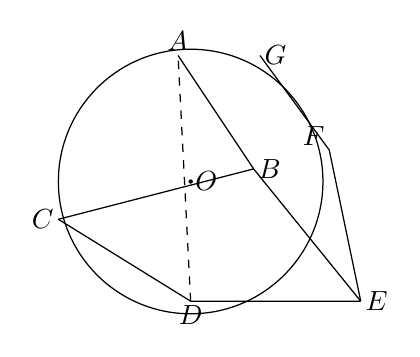
\begin{tikzpicture}[scale=0.8, line width=0.45pt,
  every node/.style={inner sep=1.5pt}]
  \coordinate (O) at (0,0); \coordinate (C) at (-2.1,-0.6); \coordinate (B) at (1.0,0.2);
  \coordinate (D) at (0.0,-1.9); \coordinate (A) at (-0.2,2.0);
  \coordinate (E) at (2.7,-1.9); \coordinate (F) at (2.2,0.5); \coordinate (G) at (1.1,2.0);
  \draw (O) circle (2.1);
  \draw (A)--(B)--(E) (C)--(D)--(E);
  \draw (E)--(F)--(G);
  \draw (C)--(B);
  \draw[dashed] (D)--(A);
  \fill (O) circle (0.035);
  \node[anchor=south] at (A) {$A$}; \node[anchor=west] at (B) {$B$};
  \node[anchor=east] at (C) {$C$}; \node[anchor=north] at (D) {$D$};
  \node[anchor=west] at (E) {$E$}; \node[anchor=south east] at (F) {$F$};
  \node[anchor=west] at (G) {$G$}; \node[anchor=west] at (O) {$O$};
\end{tikzpicture}
